%!TEX encoding = UTF-8 Unicode
\documentclass[12pt]{article} 
\usepackage[left=0.75in,top=0.7in,right=0.75in,bottom=0.3in]{geometry} % Document margins
\usepackage{CJK}
\usepackage{graphicx}
\usepackage{mathtools}
\usepackage{mathrsfs}
\usepackage{amssymb}
\usepackage{hyperref}

\makeatletter
\renewenvironment{itemize}
{\list{$\bullet$}{\leftmargin\z@ \labelwidth\z@ \itemindent-\leftmargin
\let\makelabel\descriptionlabel}}
{\endlist}
\makeatother

\begin{CJK}{UTF8}{bsmi}
\title{\textbf{Homework2 / Linear Filter}}
\author{\textbf{李豪韋 (HW-Lee) ID 103061527}}
\date{}

\begin{document}
\vspace*{-60pt}
    {\let\newpage\relax\maketitle}

\section*{Overview}
\vspace{-20pt}
\noindent\makebox[\linewidth]{\rule{\textwidth}{0.4pt}}
\vspace{5pt}

In this homework, the goal is to implement the stochastic gradient descent method (SGD, also known as LMS) that is covered extensively in class, by Hinton, and also in Haykin’s textbook. It will be applied with real data ($\mathsf{GradeData\_HW2.csv}$) as well as fake data generated by the function $\mathsf{getFakeData()}$.

The real data are basically the same data given to you in $\mathsf{HW1}$, but the $\mathsf{.csv}$ file now also includes the total score. The fake data are randomly generated via {\it principal component analysis} (PCA) to have the same 1st and 2nd-order statistics as the real data.

More specifically, the mission is to find out a set of linear combination weights that best predict the total score out of individual activities (i.e., columns).

Before proceeding to implement SGD, note that the true weights can be directly inferred by solving a pseudo inverse problem in the common least-square sense. This least-square procedure is coded at line 16 of $\mathsf{Hw2\_Starter.m}$:
\begin{center}
	$\mathsf{w\_ls = inv(inp'*inp)*(inp'*des);}$
\end{center}

Therefore, with this in mind, the result would include comparison between the weights obtained by SGD and the {\bf true} weight $\mathsf{w\_ls}$. Hopefully the weights given by SGD will converge to $\mathsf{w\_ls}$ in the stochastic sense.

\section*{Implementation}
\vspace{-20pt}
\noindent\makebox[\linewidth]{\rule{\textwidth}{0.4pt}}

\begin{enumerate}
	\item {\bf Functions}
	\begin{itemize}
		\item {\bf Hw2LinearFilter.train(X, y)} \\ \\
			Return a reference of a linear predictor trained with training set $X$ and corresponded ground truths $y$. \\
		\item {\bf Hw2LinearFilter.predict(X)} \\ \\
			Return a vector of values corresponding to unknown testing set $X$. \\
		\item {\bf Hw2LinearFilter.visualInfo()} \\ \\
			Show the property of the predictor in a visual way, including parameters $w$, $b$, and all $w$'s, $b$'s, and $e$'s during training process.
	\end{itemize}
	
	\newpage
	\item {\bf Process}
	\begin{itemize}
		\item {\bf Initialize the weights}
		\item {\bf Update the weights with error until terminated condition is satisfied}
			\begin{align*}
				&\text{In batch-mode:  }
				w = w - \eta (-\frac{1}{N}\displaystyle\sum_i (d_i - y_i) x^{(i)}) \\
				&\text{In online-mode:  }
				w = w + \eta (d-y) x
			\end{align*}
		\hspace*{-1em}
		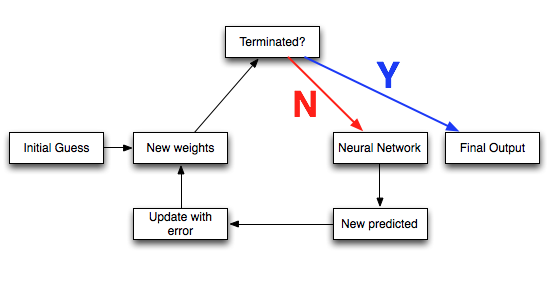
\includegraphics[scale=.8]{../res/training_algorithm.png}
	\end{itemize}
\end{enumerate}

\section*{Results}
\vspace{-20pt}
\noindent\makebox[\linewidth]{\rule{\textwidth}{0.4pt}}

\hspace*{-5em}
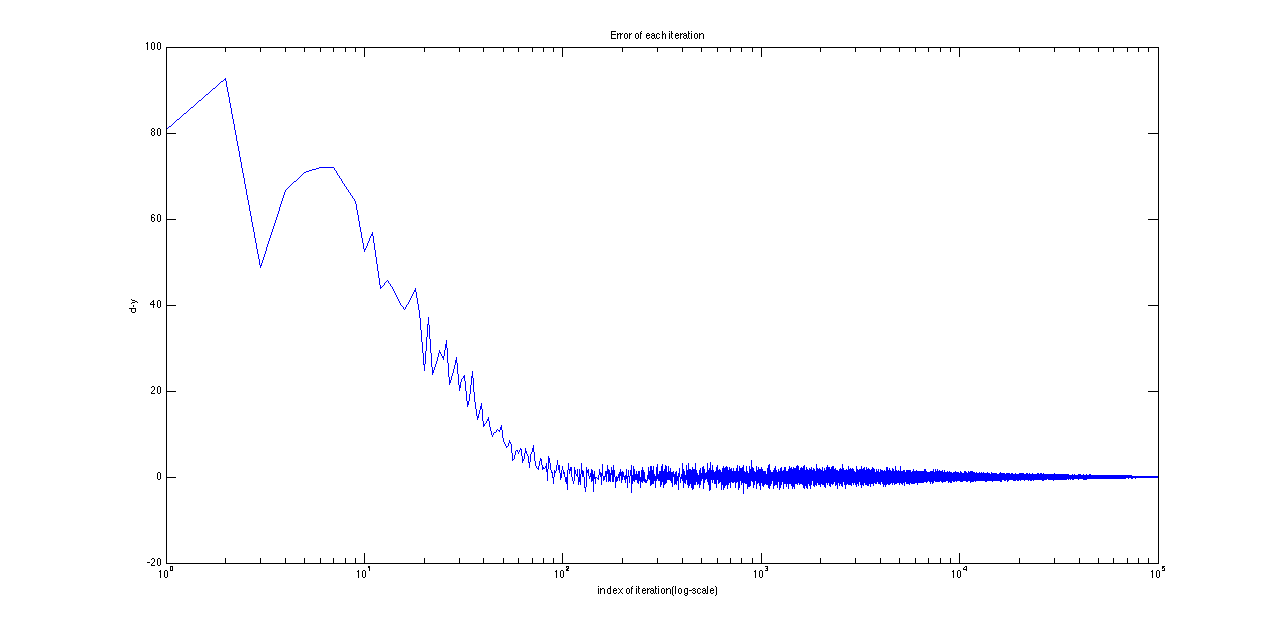
\includegraphics[scale=.45]{../res/error.png}
\begin{center}
	[Fig.1: Error value (d$-$y) w.r.t. iteration index]
\end{center}

\hspace*{-6em}
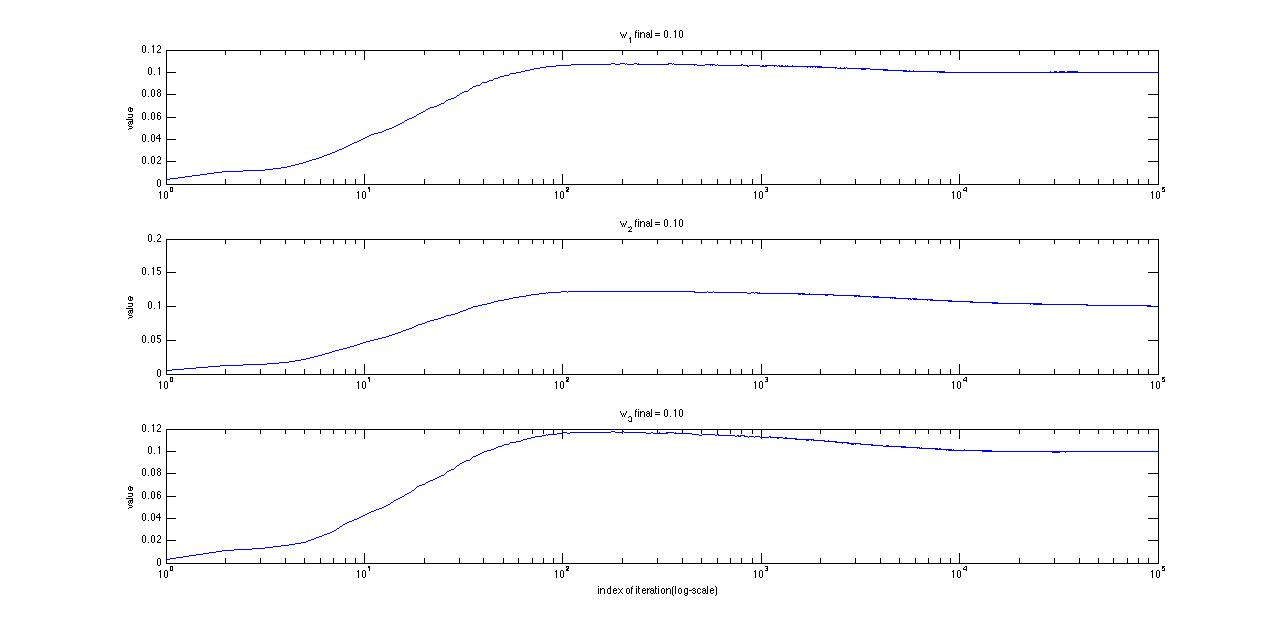
\includegraphics[scale=.25]{../res/parametrogram1.png}
\hspace*{-2.5em}
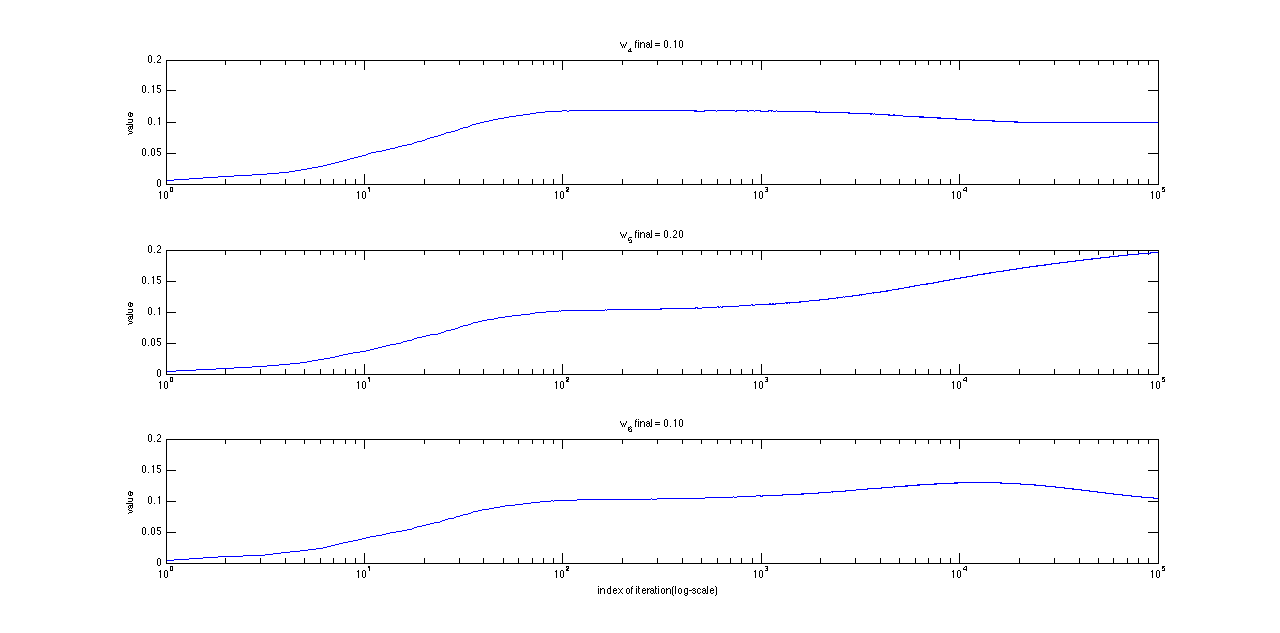
\includegraphics[scale=.25]{../res/parametrogram2.png}
\hspace*{1.5em}
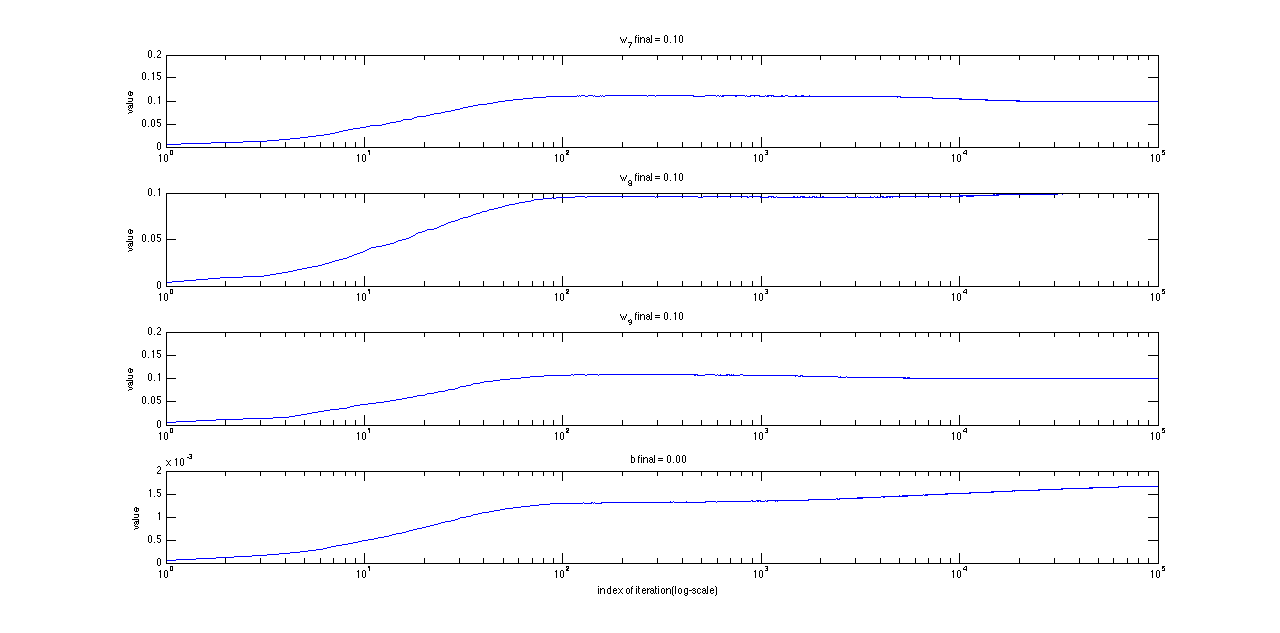
\includegraphics[scale=.35]{../res/parametrogram3.png}
\begin{center}
	[Fig.2: Parametrogram of the linear filter]
\end{center}

The figures above are: 1) difference between desired and predicted value v.s. iteration index plot, note that the x-axis is log-scale (for ease of observing the decreasing trajectory); and 2) parameters of the linear filter v.s. iteration index, respectively. They have proved that the linear filter did work, being able to decrease the difference between desired and predicted values, and will get converged as the iteration time gets larger. In the results, $\eta$ is given with $7e-7$, $1e5$ iterations, and the final weights are
$w_\text{online} = \begin{pmatrix} 0.1001 & 0.1006 & 0.0998 & 0.0997 & 0.1961 & 0.1043 & 0.0996 & 0.0998 & 0.1001 \end{pmatrix}^T$, 
$w_\text{batch} = \begin{pmatrix} 0.0999 & 0.0999 & 0.1000 & 0.0997 & 0.1956 & 0.1041 & 0.0993 & 0.0997 & 0.1001 \end{pmatrix}^T$.

\section*{Discussion}
\vspace{-20pt}
\noindent\makebox[\linewidth]{\rule{\textwidth}{0.4pt}}

\begin{enumerate}
	\item How much does your weight vector deviate from the {\bf true} weight $\mathsf{w\_ls}$?
	\begin{flushleft}
		After iterating the training algorithm with a large enough times, the weight vector will be very 'close' to $\mathsf{w\_ls}$.
	\end{flushleft}
	\newpage
	\item What is the maximal learning rate ($\eta$) you can allow before the system becomes unstable? 
		Can this only be found by {\bf trial and error}? Or is there a guideline for the choice of an appropriate learning rate?
	\begin{flushleft}
		I simply calculate the trace of $X^TX$: (Use MATLAB command $\mathsf{sum(diag(X'*X))}$), and the 'conservative' convergence upper bound $\frac{2}{tr[R_x]} = 3.0873e-07$. Therefore, there is a strategy determining the value of learning rate: $\eta$ should be close to the convergence upper bound and can be slightly larger than it to reduce the number of iterations needed to get the weights converged.
	\end{flushleft}
	\item Is there a trade off between the learning rate and how small the approximation error can get?
	\hspace*{-6em}
	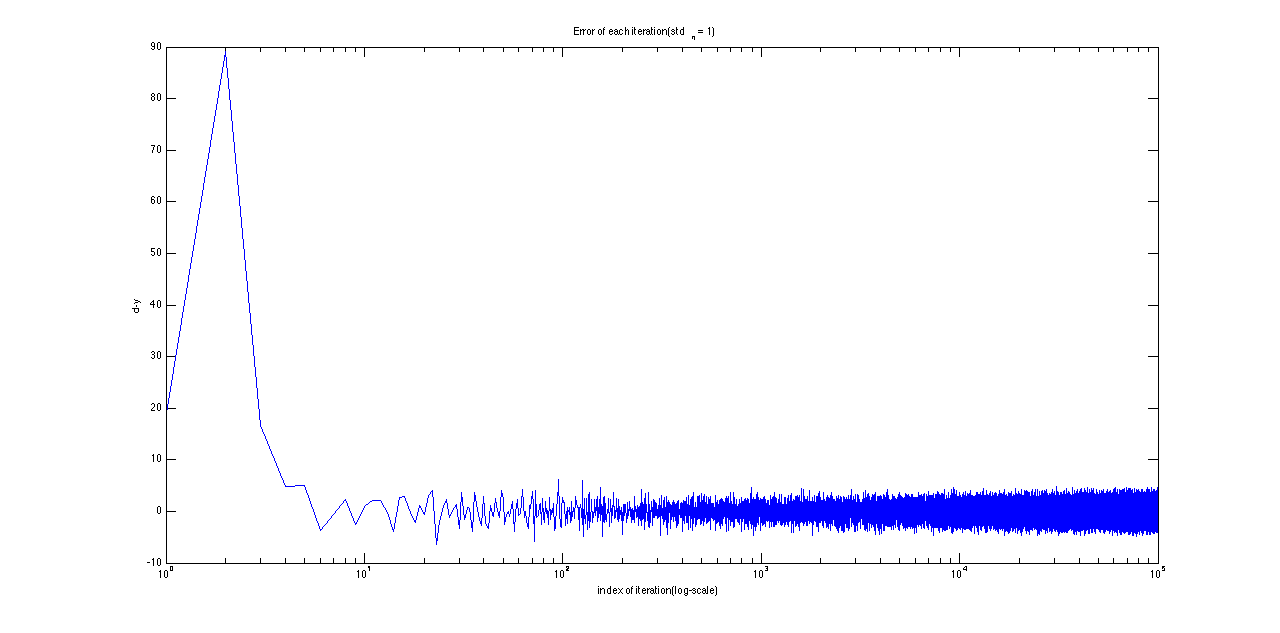
\includegraphics[scale=.25]{../res/error_std1_eta5.png}
	\hspace*{-2.5em}
	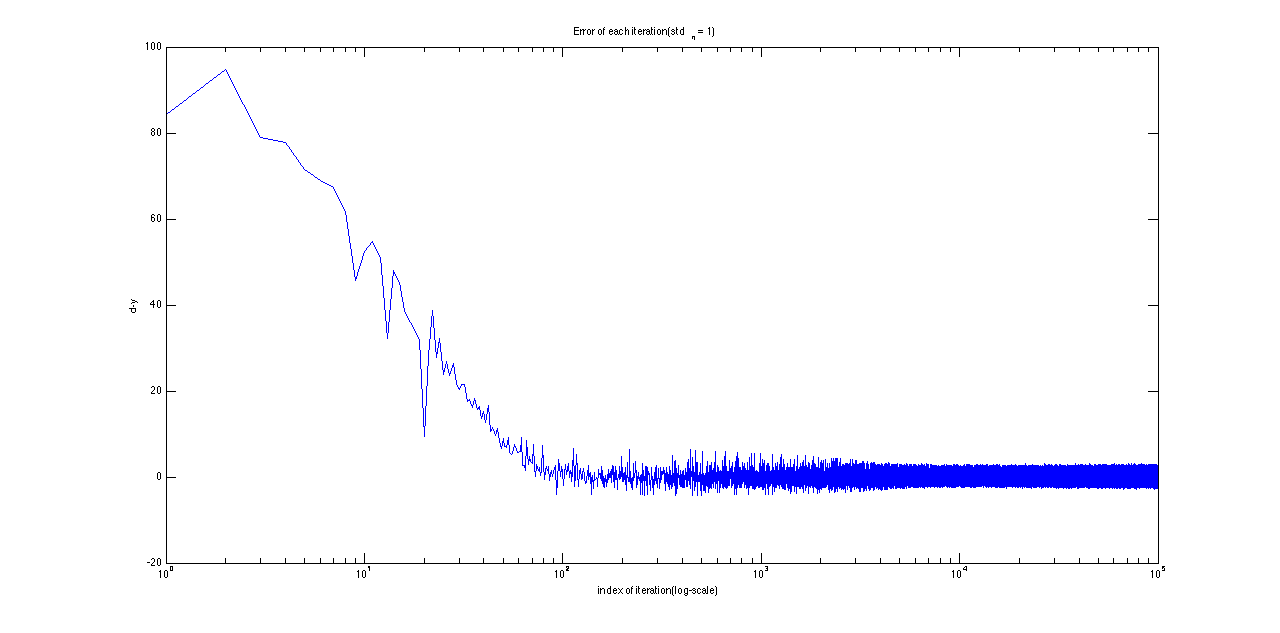
\includegraphics[scale=.25]{../res/error_std1_eta7-7.png}
	\begin{flushleft}
		Take the original training data plus standard deviation 1 noise for example: the left-side figure is applied with learning rate $1e-5$ while the right-side figure is applied with $7e-7$. Obviously, the error margin of the right-side figure is smaller than the right-side. Then, we can conclude that the increase of learning rate will accelerate the speed of convergence while sacrifice the error margin after large iterations.
	\end{flushleft}
	\item When sampling the real data, does it help to keep drawing the samples randomly?
	\begin{flushleft}
		In practice, this operation can only accelerate the speed of convergence. (It will be discussed more specifically below)
	\end{flushleft}
	\item (Continuing from above) If so, does it help to draw the samples repeatedly in the same order?
	\begin{flushleft}
		Yes. Under a large iteration time, the weights will get converged in any way.
	\end{flushleft}
	\item In the for-loop, how would the performance be changed if the observation vector $\mathsf{d}$ is subject to additive noise? 
		E.g., let $\mathsf{d = d + randn(5, 0)}$ under a predefined standard deviation $\sigma = 5.0$. Would SGD fail to converge? 
		Would the performance degrade? 
		\begin{flushleft}
			According to the Figure.3 and Figure.4 below, it is possible that SGD will fail to converge when noise is added. Form.1 shows the error with various noise (different standard deviation), and we can know std of noise is positively correlated to error.
		\end{flushleft}
		\begin{center}
			More detailed implementation is available on \href{https://github.com/HW-Lee/2015-NN-Homeworks}{$\mathsf{https://github.com/HW}$-$\mathsf{Lee/2015}$-$\mathsf{NN}$-$\mathsf{Homeworks}$}.
		\end{center}
	\hspace*{-4em}
	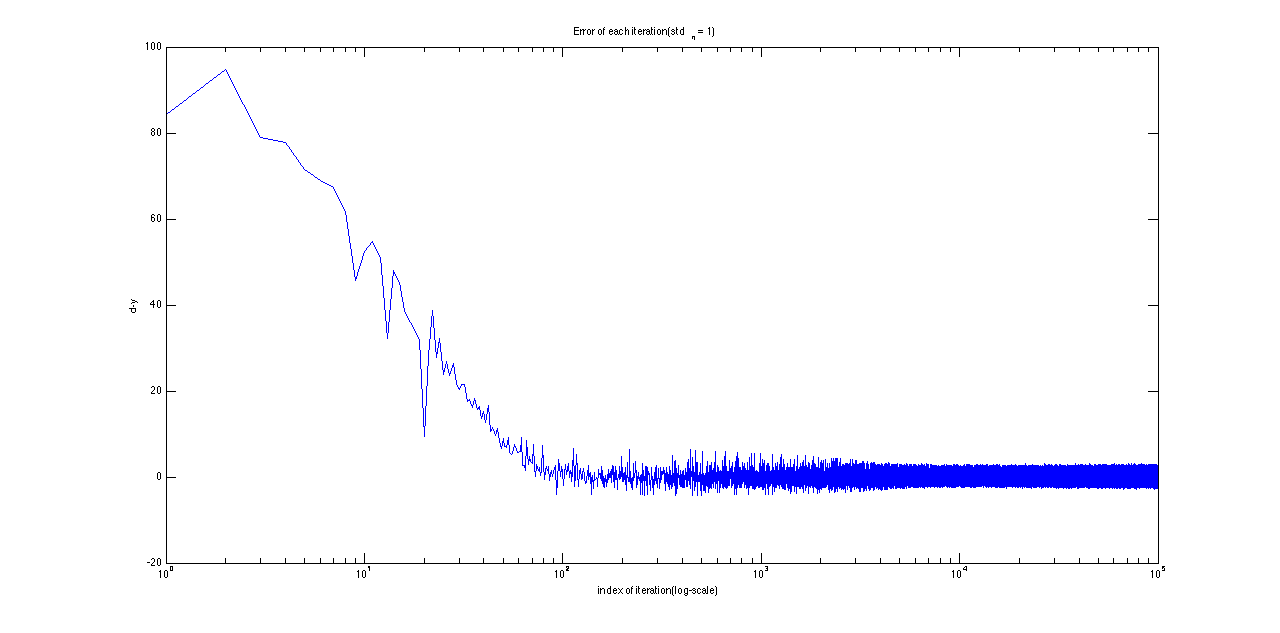
\includegraphics[scale=.45]{../res/error_std1_eta7-7.png}
	\begin{center}
		[Fig.3: Error w.r.t. iteration index with signal plus 1 std noise]
	\end{center}
	\hspace*{-4em}
	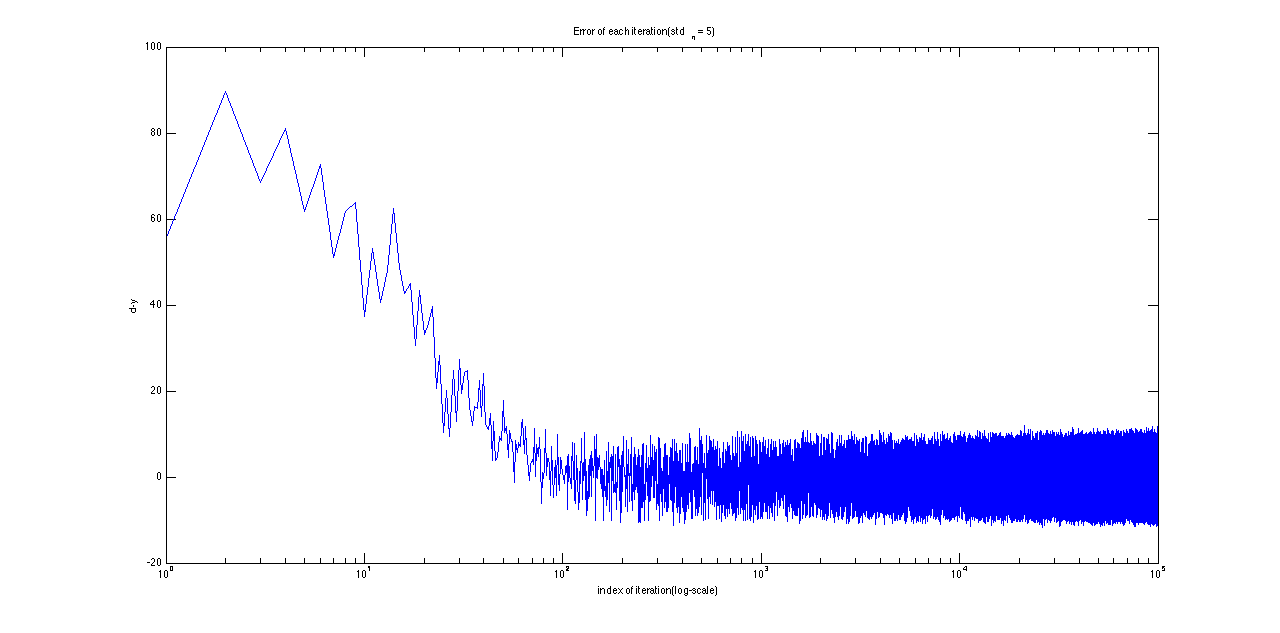
\includegraphics[scale=.45]{../res/error_std5_eta7-7.png}
	\begin{center}
		[Fig.4: Error w.r.t. iteration index with signal plus 5 std noise]
	\end{center}
	\begin{center}
		\begin{tabular}{|c|c|c|c|c|c|}
			\hline
			$\sigma$ & 1 & 2 & 3 & 4 & 5 \\
			\hline
			$\epsilon$ & $0.7227\pm 0.3937$ & $1.5506\pm 0.9835$ & $2.1620\pm 1.1115$ & $2.3936\pm 1.2747$ & $3.0411\pm 1.5018$ \\
			\hline
		\end{tabular}
		
		[Form.1: Error with various noise added]
	\end{center}
	
\end{enumerate}

\section*{Additional Discussion: \\ Results from batch-mode and online-mode}
\vspace{-20pt}
\noindent\makebox[\linewidth]{\rule{\textwidth}{0.4pt}}

\hspace*{-11em}
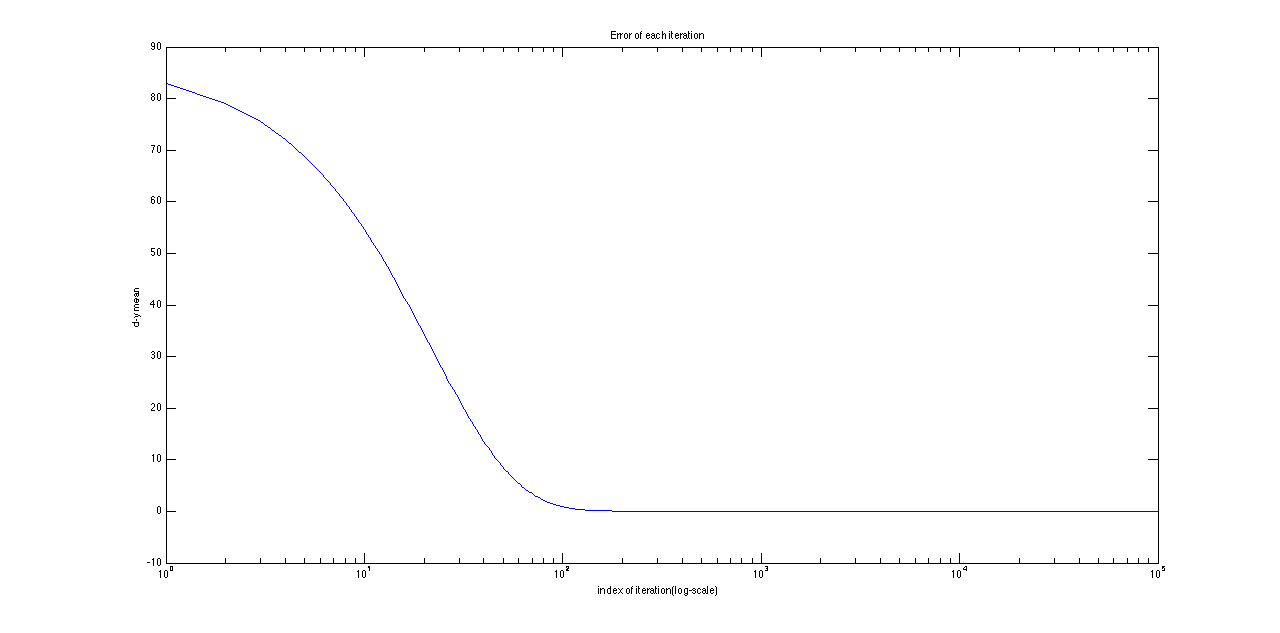
\includegraphics[width=25cm, height=8.7cm]{../res/error_batch.png}
\hspace*{-9.4em}
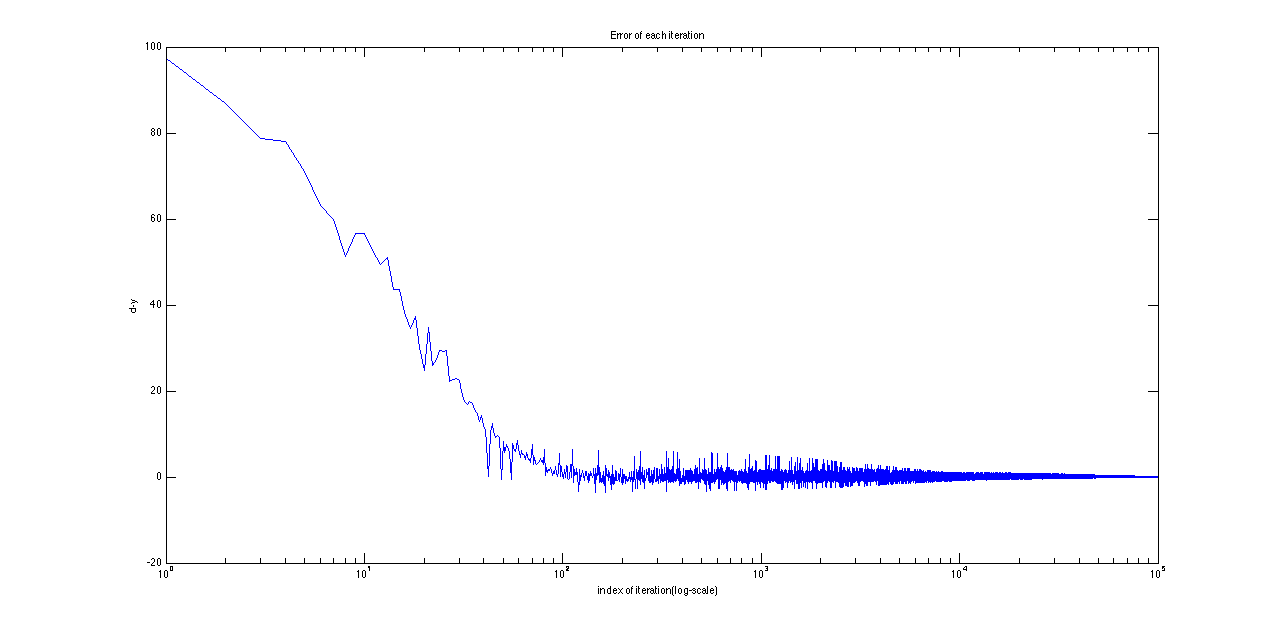
\includegraphics[width=25cm, height=8.7cm]{../res/error_online.png}

In this section, there are two figures shown above: 1) the upper one shows error value with batch-mode, and 2) the lower one shows with online-mode . According to these figures, we can get:
\begin{itemize}
	\item The speed of convergence is not significantly different in these two different method.
	\item The error curve is smoother in batch-mode than in online-mode, because batch-mode updates weights after looking through all data.
	\item Batch-mode trains the linear filter by repeatedly feeding the whole data {\bf in the same order}, it shows that the $5^{thit}$ question in discussion section is true.
	\item Followed by above, batch-mode also shows that randomly sampling from real data cannot change the performance we finally get. (the $4^{th}$ question in discussion section) 
\end{itemize}

\end{CJK}
\end{document}